\section{Supporting figures}

\begin{figure}[H]
\centering
\begin{tabular}{c}
\begin{subfigure}[b]{\textwidth}
  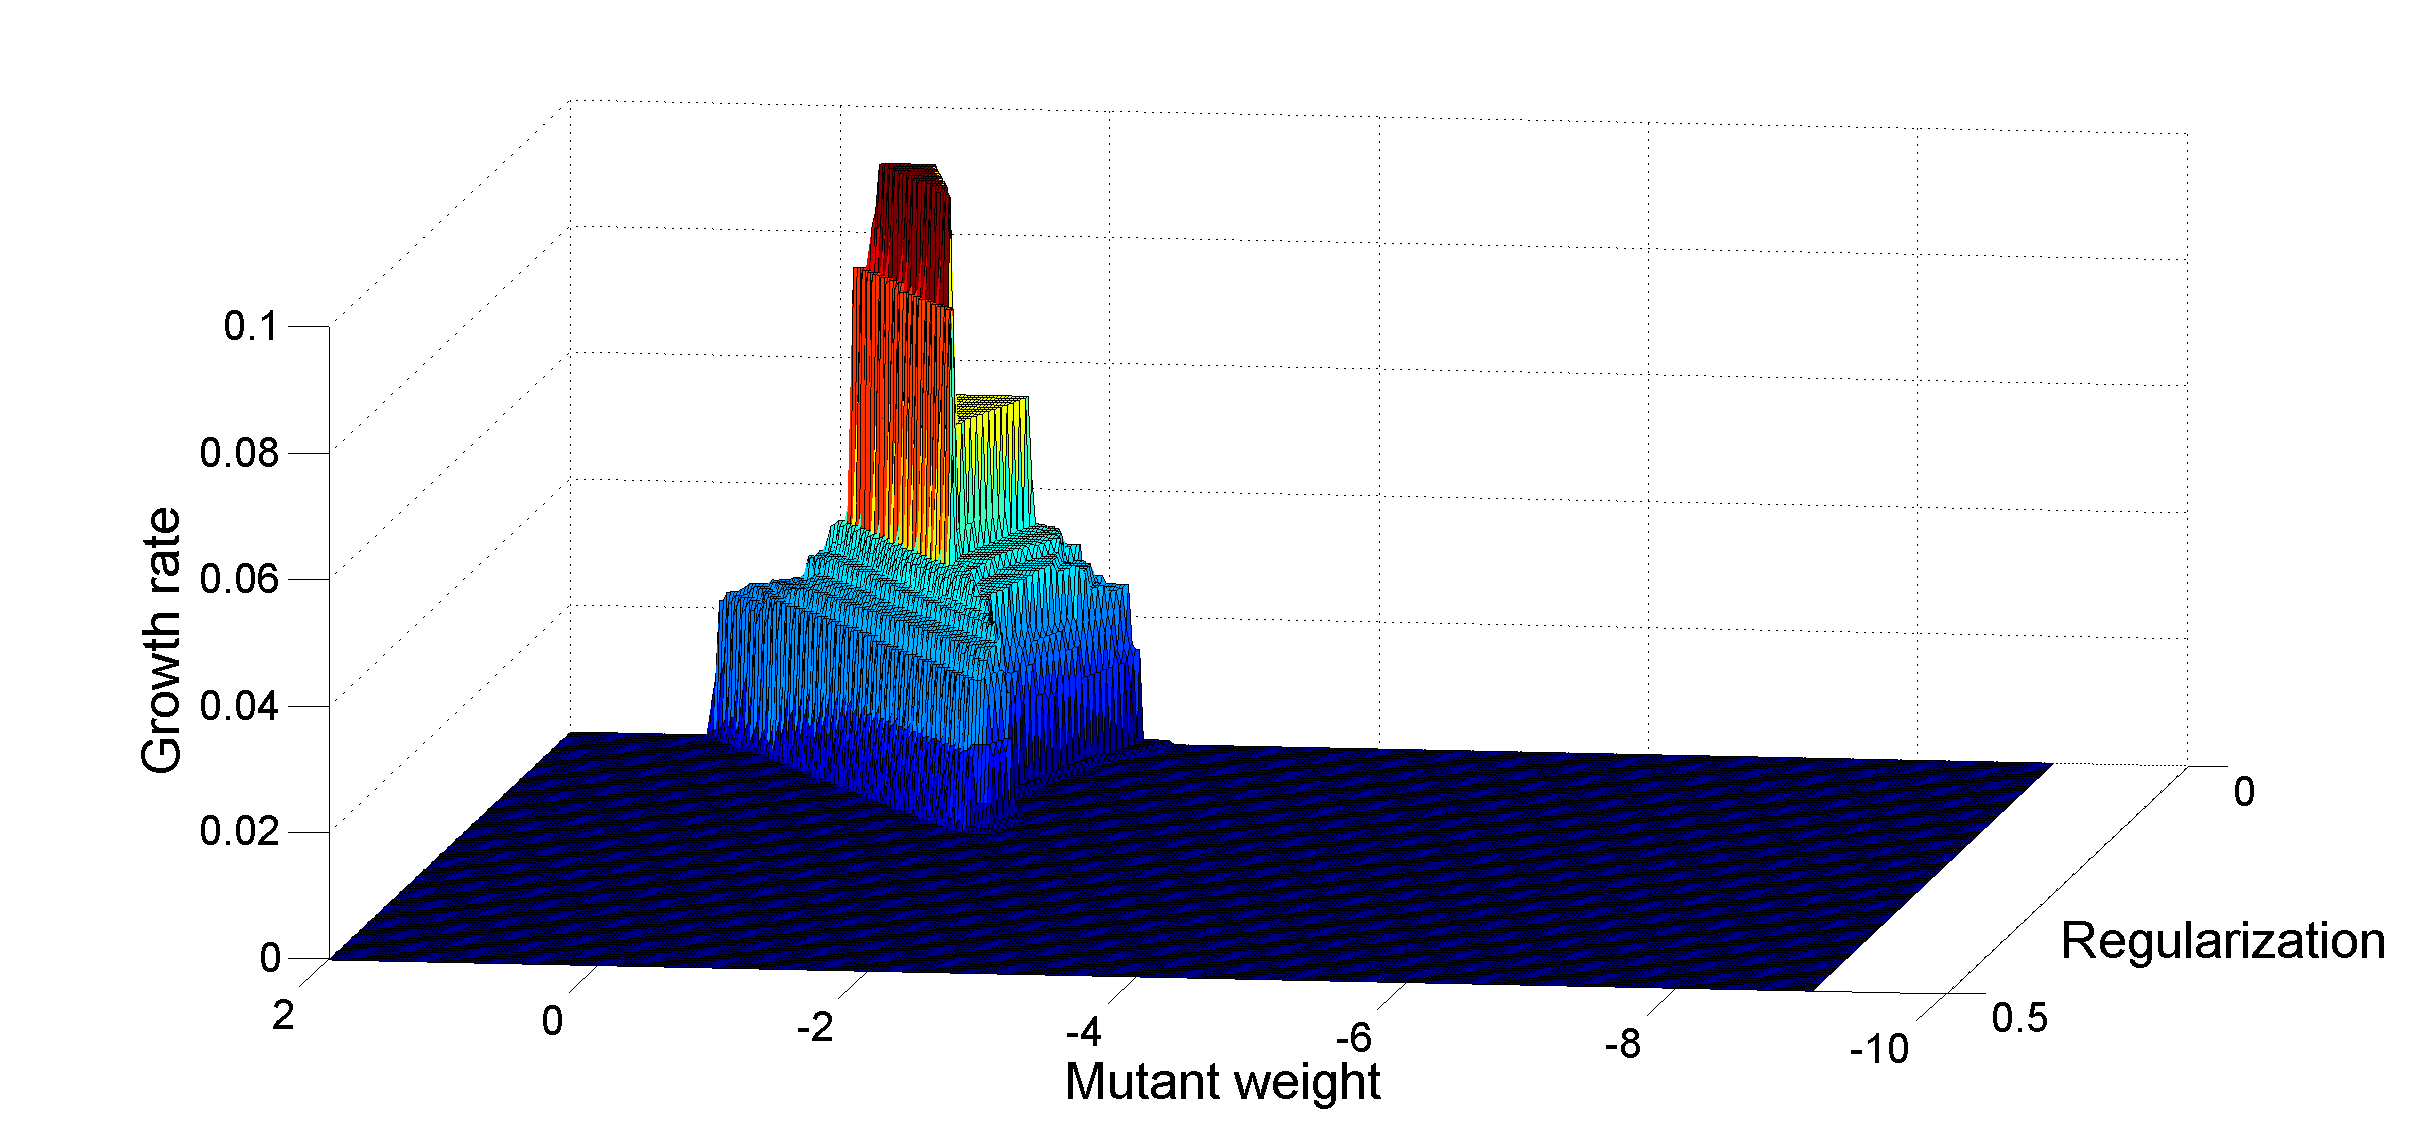
\includegraphics[width=\textwidth]{R264LP}
  \caption{Linear MoMA} 
  \label{fig:R264LP}
\end{subfigure}
\\
\begin{subfigure}[b]{\textwidth}
  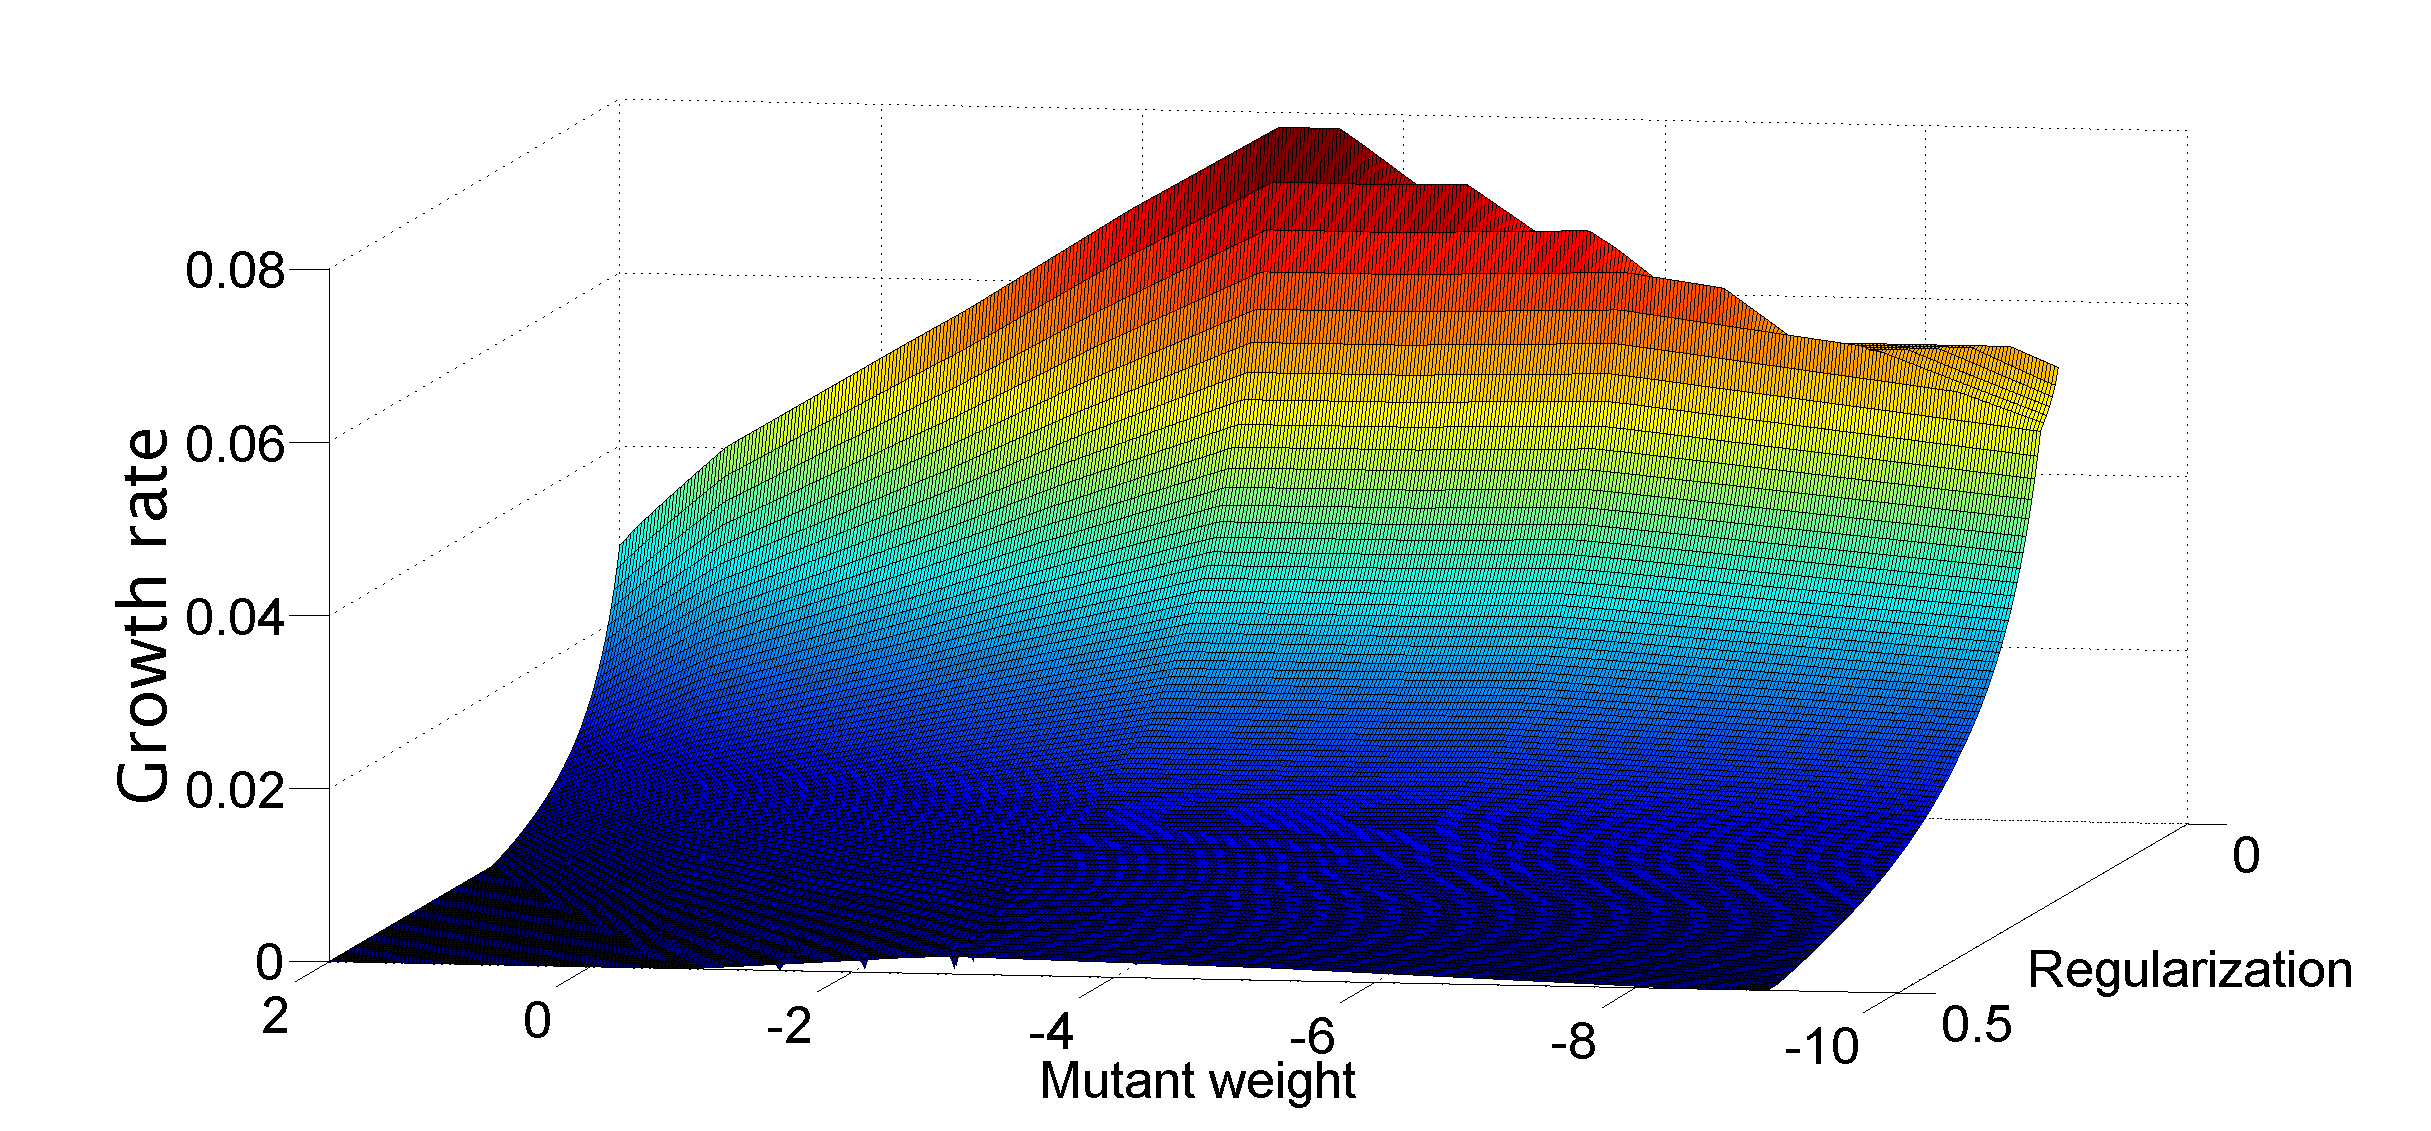
\includegraphics[width=\textwidth]{R264QP}
  \caption{Quadratic MoMA} 
  \label{fig:R264QP}
\end{subfigure}
\\
\end{tabular}
\caption{The same reaction is used in both figures, and in both
instances, a slightly negative weight on the reaction appears to be
most beneficial (compare to 0, which represents the wild-type).
Weight on a (linear or quadratic, respectively) 
regularization objective component is shown on the y-axis, which is often a helpful
constant both biologically and for removing invalid flux cycles 
\citep{Schuetz2012, Smallbone2009a}.}
\label{fig:wMoMA_smoothness}
\end{figure}

\begin{figure}[H]
\centering
  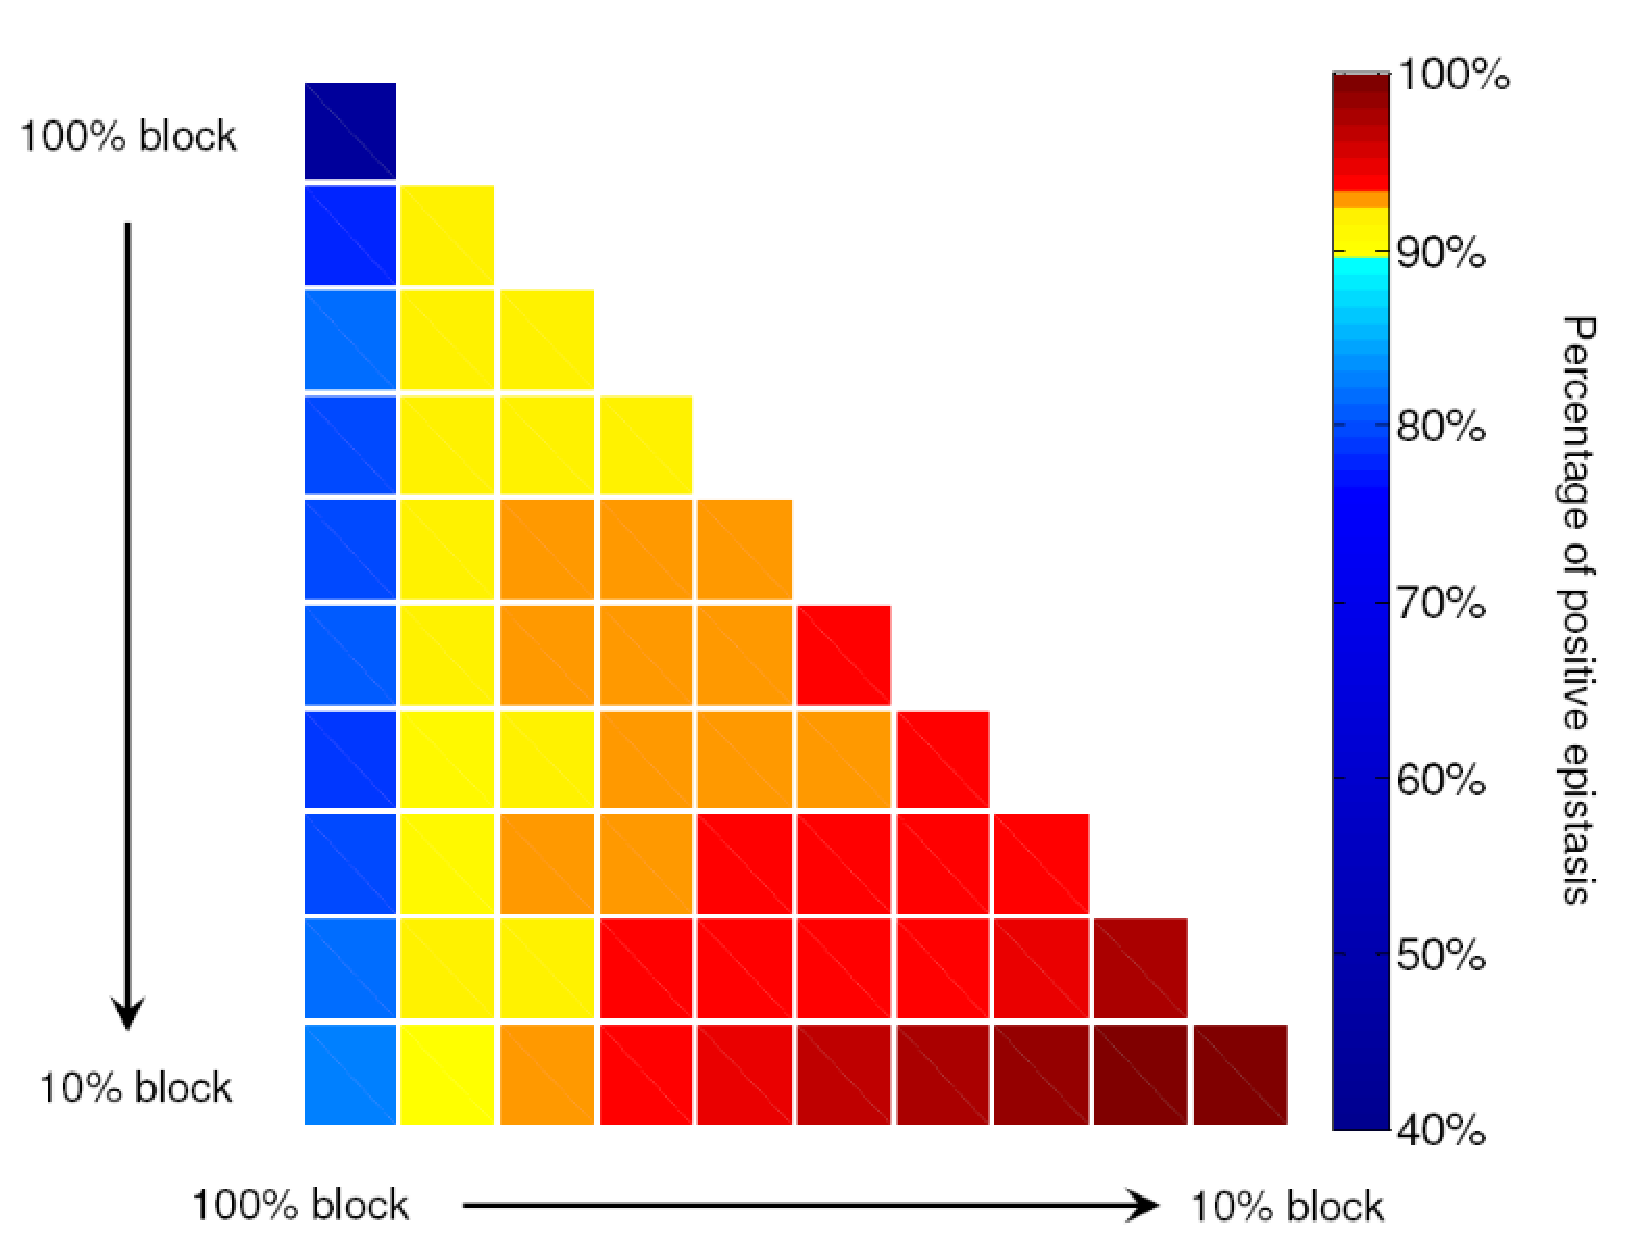
\includegraphics[width=\textwidth]{deleteriousYeastEpiLandscape}
  \caption{Flux restriction increases the percentage of negative
  epistasic interactions. Data taken from \citet{Xu2012}.}
  \label{fig:delYeastEpiLandscape}
\end{figure}

\begin{figure}[H]
\centering
\begin{tabular}{c}
\begin{subfigure}[b]{\textwidth}
  \includegraphics[width=\textwidth]{50_mut_YPE_tmp}
  \caption{50\% Gaussian sampling} 
  \label{fig:beneEpiPairwise:50}
\end{subfigure}
\\
\begin{subfigure}[b]{\textwidth}
  \includegraphics[width=\textwidth]{uni_mut_YPE_tmp}
  \caption{Uniform sampling}
  \label{fig:beneEpiPairwise:uni}
\end{subfigure}
\\
\end{tabular}
\caption{Example distributions of beneficial mutations for the yeast
YPE example when sampling 50\% of flux mutations within the larger FVA
bound using a truncated normal distribution
\textbf(\ref{fig:beneEpiPairwise:50}) or when using uniform sampling
between the FVA bounds \textbf(\ref{fig:beneEpiPairwise:uni}).}
\label{fig:50andUniSampling}
\end{figure}


\section{Supporting information}

\subsection{Evolutionary path analysis}
\label{sec:pathAnalysis}

The repository housing the project is currently located at:
\url{https://github.com/bbarker/COBRAscripts}. The C code which is
used for the analysis may be found in the
\texttt{MyProjects/AdaptiveMuts/TreeTraversal} subdirectory. 


%
% First entry in 
% /home/brandon/FBA/models/Analysis/AdaptiveMOMA/simulationsMM15pLM/
% 4xMM_1_1k_grRateMat.csv
%

The power-set of mutations can be ordered in the natural binary order.
For instance, four mutations can be ordered from $0000$ (wild-type) to
$1111$ (all mutations present) , where a '0' denotes the absence of
the given mutation and a '1' denotes its presence. An example of the
four mutation case can be given in one line of a text file as follows:

\vspace{1ex}
\noindent
\texttt{0.013743, 0.024794, 0.020672, 0.023515, 0.019147, 0.02291, 0,
0, 0.017884, 0.024196, 0.016066, 0.023515, 0.015166, 0.02291, 0, 0}
\vspace{1ex}


The first fitness in the list, which corresponds to the wild-type, is
the divisor in the following output from
\texttt{printPaths}\footnote{\texttt{printpaths} has the same usage as
\texttt{trapFind}; see page \pageref{trapFindCmd}}, showing all $4!$
paths that may arise from the above mutants.

\begin{verbatim}
*** Replicate 0 ***
0       4       3       2       1
1.000000        1.301317        1.103544        0.000000        0.000000
0       4       3       1       2
1.000000        1.301317        1.103544        1.667030        0.000000
0       4       2       3       1
1.000000        1.301317        1.169032        0.000000        0.000000
0       4       2       1       3
1.000000        1.301317        1.169032        1.711053        0.000000
0       4       1       3       2
1.000000        1.301317        1.760605        1.667030        0.000000
0       4       1       2       3
1.000000        1.301317        1.760605        1.711053        0.000000
0       3       4       2       1
1.000000        1.393218        1.103544        0.000000        0.000000
0       3       4       1       2
1.000000        1.393218        1.103544        1.667030        0.000000
0       3       2       4       1
1.000000        1.393218        0.000000        0.000000        0.000000
0       3       2       1       4
1.000000        1.393218        0.000000        0.000000        0.000000
0       3       1       4       2
1.000000        1.393218        1.667030        1.667030        0.000000
0       3       1       2       4
1.000000        1.393218        1.667030        0.000000        0.000000
0       2       4       3       1
1.000000        1.504184        1.169032        0.000000        0.000000
0       2       4       1       3
1.000000        1.504184        1.169032        1.711053        0.000000
0       2       3       4       1
1.000000        1.504184        0.000000        0.000000        0.000000
0       2       3       1       4
1.000000        1.504184        0.000000        0.000000        0.000000
0       2       1       4       3
1.000000        1.504184        1.711053        1.711053        0.000000
0       2       1       3       4
1.000000        1.504184        1.711053        0.000000        0.000000
0       1       4       3       2
1.000000        1.804118        1.760605        1.667030        0.000000
0       1       4       2       3
1.000000        1.804118        1.760605        1.711053        0.000000
0       1       3       4       2
1.000000        1.804118        1.667030        1.667030        0.000000
0       1       3       2       4
1.000000        1.804118        1.667030        0.000000        0.000000
0       1       2       4       3
1.000000        1.804118        1.711053        1.711053        0.000000
0       1       2       3       4
1.000000        1.804118        1.711053        0.000000        0.000000
\end{verbatim}

'Replicate 0' merely denotes that this output was due to the first
example power set of mutants in a file, since
\texttt{randomBeneficialPsets.m} or \texttt{randomAdaptivePsets.m} can
be used to generate multiple sets of mutants. The primary difference
between the two scripts is that the former uses hard constraint
changes as mutations, whereas the latter uses weights (which is the
version used in the present study).  In an experimental setting,
it is much more likely that we would only have one replicate, which is
exactly why experimental settings are unlikely to be useful for
showing trends in adaptive evolution. Each line of fitnesses is
preceded by a corresponding line which lists which mutation was added
at that point in the evolutionary path (0 to $n$ where $n$ is the
number of mutations, so $n = 4$ in this example). It may be desirable 
to map these mutations back to the reactions they are asssociated with
in the model. This output from the above scripts is stored in files
with the suffix \texttt{\_rxnlist.csv}.

The \texttt{trapFind} program can be used to find how many paths have
traps (local fitness optima or fitness decreases) that prevent
adaptation from reaching the global fitness maximum among all
combinations of mutations in the set.

This program takes as its first argument a file containing comma-delimited 
lists of mutant fitneses described above, followed by the number of 
individual mutations as the second argument, and the number of replicats 
(lines in the file) as the third argument:

\vspace{1ex}
\noindent
\texttt{trapFind [number of mutants] [number of replicates]}
\label{trapFindCmd}
\vspace{1ex}
 
The output is contained in \texttt{[original file
prefix]\_trapAnalysis.csv}. The contents of the file are
comma-separated lists (one per mutation set) that have the following
information: number of mutations, number of paths that reach the
optimium, number paths terminated due to a decrease in fitness, and
the number of paths terminated due to local maxima. As a further
example, the output for three experimental datasets has been listed
(Table~\ref{tab:threeAdaptEvoDats}).

\begin{table}
\centering
\begin{tabular}{ccccc}
study                 & mutations & reached optima & trap: fitness decrease & trap: local maxima \\
\citet{Weinreich2006} & 5         & 96             & 18                     & 0                  \\
\citet{Khan2011}      & 5         & 108            & 7                      & 0                  \\
\citet{Chou2011}      & 4         & 24             & 0                      & 0                  \\
\end{tabular}
\caption{Example output of \texttt{trapFind} applied to experimental
datasets. The input files may be found in this project's
\texttt{TreeTraversal/Experiments} subdirectory.}
\label{tab:threeAdaptEvoDats}
\end{table}

Note that some paths that become trapped may have themselves branched
into other paths, so the tally for the last three columns does not
necessarily reach $n!$. If we consider that neutral mutations are
unlikely to become fixed in a population \citep{Weinreich2006}, only
18 of 120 paths are evolutionarily inaccessible, instead of the 96
encountered in this analysis.

\subsection{Pairwise adaptive mutations}

The function we used to generate the pairwise
epistasis data is \texttt{randomEpistasisSampler} found in 
\texttt{MyProjects/AdaptiveMuts}. This function relies on another
function in the same directory for generating a pool of single
mutants, \texttt{randomSingleBeneMuts}.

